% Options for packages loaded elsewhere
% Options for packages loaded elsewhere
\PassOptionsToPackage{unicode}{hyperref}
\PassOptionsToPackage{hyphens}{url}
\PassOptionsToPackage{dvipsnames,svgnames,x11names}{xcolor}
%
\documentclass[
  letterpaper,
  sfsidenotes]{tufte-book}
\usepackage{xcolor}
\usepackage{amsmath,amssymb}
\setcounter{secnumdepth}{-\maxdimen} % remove section numbering
\usepackage{iftex}
\ifPDFTeX
  \usepackage[T1]{fontenc}
  \usepackage[utf8]{inputenc}
  \usepackage{textcomp} % provide euro and other symbols
\else % if luatex or xetex
  \usepackage{unicode-math} % this also loads fontspec
  \defaultfontfeatures{Scale=MatchLowercase}
  \defaultfontfeatures[\rmfamily]{Ligatures=TeX,Scale=1}
\fi
\usepackage{lmodern}
\ifPDFTeX\else
  % xetex/luatex font selection
  \setmainfont[]{ETbb}
  \setsansfont[Scale=MatchUppercase]{TeX Gyre Heros}
\fi
% Use upquote if available, for straight quotes in verbatim environments
\IfFileExists{upquote.sty}{\usepackage{upquote}}{}
\IfFileExists{microtype.sty}{% use microtype if available
  \usepackage[]{microtype}
  \UseMicrotypeSet[protrusion]{basicmath} % disable protrusion for tt fonts
}{}
% Make \paragraph and \subparagraph free-standing
\makeatletter
\ifx\paragraph\undefined\else
  \let\oldparagraph\paragraph
  \renewcommand{\paragraph}{
    \@ifstar
      \xxxParagraphStar
      \xxxParagraphNoStar
  }
  \newcommand{\xxxParagraphStar}[1]{\oldparagraph*{#1}\mbox{}}
  \newcommand{\xxxParagraphNoStar}[1]{\oldparagraph{#1}\mbox{}}
\fi
\ifx\subparagraph\undefined\else
  \let\oldsubparagraph\subparagraph
  \renewcommand{\subparagraph}{
    \@ifstar
      \xxxSubParagraphStar
      \xxxSubParagraphNoStar
  }
  \newcommand{\xxxSubParagraphStar}[1]{\oldsubparagraph*{#1}\mbox{}}
  \newcommand{\xxxSubParagraphNoStar}[1]{\oldsubparagraph{#1}\mbox{}}
\fi
\makeatother


\usepackage{longtable,booktabs,array}
\usepackage{calc} % for calculating minipage widths
% Correct order of tables after \paragraph or \subparagraph
\usepackage{etoolbox}
\makeatletter
\patchcmd\longtable{\par}{\if@noskipsec\mbox{}\fi\par}{}{}
\makeatother
% Allow footnotes in longtable head/foot
\IfFileExists{footnotehyper.sty}{\usepackage{footnotehyper}}{\usepackage{footnote}}
\makesavenoteenv{longtable}
\usepackage{graphicx}
\makeatletter
\newsavebox\pandoc@box
\newcommand*\pandocbounded[1]{% scales image to fit in text height/width
  \sbox\pandoc@box{#1}%
  \Gscale@div\@tempa{\textheight}{\dimexpr\ht\pandoc@box+\dp\pandoc@box\relax}%
  \Gscale@div\@tempb{\linewidth}{\wd\pandoc@box}%
  \ifdim\@tempb\p@<\@tempa\p@\let\@tempa\@tempb\fi% select the smaller of both
  \ifdim\@tempa\p@<\p@\scalebox{\@tempa}{\usebox\pandoc@box}%
  \else\usebox{\pandoc@box}%
  \fi%
}
% Set default figure placement to htbp
\def\fps@figure{htbp}
\makeatother





\setlength{\emergencystretch}{3em} % prevent overfull lines

\providecommand{\tightlist}{%
  \setlength{\itemsep}{0pt}\setlength{\parskip}{0pt}}



 
\usepackage[]{natbib}
\bibliographystyle{plainnat}


% FIX Marginnote duplication
\usepackage{savesym}
\savesymbol{marginfigure}
\savesymbol{marginnote}
\savesymbol{sidenote}

%%%%%%%
%  FIX Makeuppercase error
%  FIX Font clash Math error
%  See https://tex.stackexchange.com/q/202142/157312
% 

\renewcommand{\textls}[2][5]{%
  \begingroup\addfontfeatures{LetterSpace=#1}#2\endgroup
}
\renewcommand{\allcapsspacing}[1]{\textls[15]{#1}}
\renewcommand{\smallcapsspacing}[1]{\textls[10]{#1}}
\renewcommand{\allcaps}[1]{\textls[15]{\MakeTextUppercase{#1}}}
\renewcommand{\smallcaps}[1]{\smallcapsspacing{\scshape\MakeTextLowercase{#1}}}
\renewcommand{\textsc}[1]{\smallcapsspacing{\textsmallcaps{#1}}}

\PassOptionsToPackage{no-math}{fontspec}
% \usepackage[mathlf, minionint,footnotefigures, frenchmath]{MinionPro}
% \setmainfont{$$}
% \setsansfont{TeX Gyre Heros}[Scale=MatchUppercase]

\ExplSyntaxOn
\int_new:N \l_mathcode_minus_int
\int_new:N \l_mathcode_equal_int
\exp_args:Nx \AtBeginDocument {
  \exp_not:n {
    \int_set:Nn \l_mathcode_minus_int { \XeTeXmathcodenum `\- }
    \int_set:Nn \l_mathcode_equal_int { \XeTeXmathcodenum `\= }
  }
  \mathcode \int_eval:n { `\- } = \number \mathcode `\- \scan_stop:
  \mathcode \int_eval:n { `\= } = \number \mathcode `\= \scan_stop:
}
\AtBeginDocument {
  \XeTeXmathcodenum `\- = \l_mathcode_minus_int
  \XeTeXmathcodenum `\= = \l_mathcode_equal_int
}
\ExplSyntaxOff

\usepackage[italic]{mathastext}
% \setromanfont{TeX Gyre Termes}


%%%%%%%


\usepackage{pdfpages}  % for cover page
\graphicspath{{Images/}} % Make Images/ default figure path


\setlength{\parindent}{0pt}%
\setlength{\RaggedRightParindent}{0pt}
\setlength{\JustifyingParindent}{0pt}%
\setlength{\parskip}{\baselineskip}

%%
% Produces a full title page

\renewcommand{\maketitlepage}[0]{%
  \cleardoublepage%
  {%
  \sffamily%
  \begin{fullwidth}%
  \fontsize{12}{14}\selectfont\par\noindent\textcolor{darkgray}{\allcaps{\thanklessauthor}}%
  \vspace{12.5pc}%
  \fontsize{20}{28}\selectfont\par\noindent\textcolor{darkgray}{\allcaps{\thanklesstitle}}%
  \vfill%
  \fontsize{10}{12}\selectfont\par\noindent\allcaps{\thanklesspublisher}%
  \end{fullwidth}%
  }
  \thispagestyle{empty}%
  \clearpage%
}

% DEFINITIONS


% The fancyvrb package lets us customize the formatting of verbatim
% environments.  We use a slightly smaller font.
\usepackage{fancyvrb}
\fvset{fontsize=\normalsize}

%%
% Prints argument within hanging parentheses (i.e., parentheses that take
% up no horizontal space).  Useful in tabular environments.
\newcommand{\hangp}[1]{\makebox[0pt][r]{(}#1\makebox[0pt][l]{)}}

%%
% Prints an asterisk that takes up no horizontal space.
% Useful in tabular environments.
\newcommand{\hangstar}{\makebox[0pt][l]{*}}

%%
% Prints a trailing space in a smart way.
\usepackage{xspace}


% Prints the month name (e.g., January) and the year (e.g., 2008)
\newcommand{\monthyear}{%
  \ifcase\month\or January\or February\or March\or April\or May\or June\or
  July\or August\or September\or October\or November\or
  December\fi\space\number\year
}


% Prints an epigraph and speaker in sans serif, all-caps type.
\newcommand{\epigraph}[2]{%
  \begin{fullwidth}
  \begin{flushright}
  \sffamily\fontsize{8}{10}\selectfont
  \sffamily\footnotesize
  \begin{doublespace}
  \vspace{-8cm}\noindent\allcaps{#1}\\% epigraph
  \noindent\allcaps{#2}\\% author
  \end{doublespace}
  \vspace{5.1cm}
  \end{flushright}
  \end{fullwidth}
  \normalfont
}


\newcommand{\blankpage}{\newpage\hbox{}\thispagestyle{empty}\newpage}


% insert 4cm before quote
\renewenvironment{quote}{
  \list{}{\leftmargin=3.5cm\topsep=0pt}
  \item\relax\small\itshape
}
{\endlist}


%  change chapter formatting
\titlespacing*{\chapter}{0pt}{5cm}{1cm}
% \titlespacing*{\section}{0pt}{.6em}{.3em}
% \titlespacing*{\subsection}{0pt}{.4em}{.2em}

\titlespacing*{\section}{0pt}{0pt}{0pt}
\titlespacing*{\subsection}{0pt}{0pt}{0pt}


%  Change Figure Caption in the Margin size
% \renewenvironment{@tufte@margin@float}[2][-1.2ex]%
%   {\FloatBarrier% process all floats before this point so the figure/table numbers stay in order.
%   \begin{lrbox}{\@tufte@margin@floatbox}%
%   \begin{minipage}{\marginparwidth}%
%     \@tufte@caption@font\footnotesize% <-- Add fontnotesize
%     \def\@captype{#2}%
%     \hbox{}\vspace*{#1}%
%     \@tufte@caption@justification%
%     \@tufte@margin@par%
%     \noindent\normalsize%<-- restored size
%   }
%   {\end{minipage}%
%   \end{lrbox}%
%   \marginpar{\usebox{\@tufte@margin@floatbox}}%
  % }


% \renewcommand\footnotesize{%
%    \@setfontsize\footnotesize\@viiipt{9}%
%    \abovedisplayskip 5\p@ \@plus2\p@ \@minus4\p@
%    \abovedisplayshortskip \z@ \@plus\p@
%    \belowdisplayshortskip 2.8\p@ \@plus\p@ \@minus2\p@
%    \def\@listi{\leftmargin\leftmargini
%                \topsep 2.5\p@ \@plus\p@ \@minus\p@
%                \parsep 2\p@ \@plus\p@ \@minus\p@
%                \itemsep \parsep}%
%    \belowdisplayskip \abovedisplayskip
% }

% % Define Tuftian float styles (with the caption in the margin)
% \newcommand{\floatc@tufteplain}[2]{%
% \begin{lrbox}{\@tufte@caption@box}%
%   \begin{minipage}[\floatalignment]{\marginparwidth}\hbox{}%
%     \footnotesize\@tufte@caption@font{\@fs@cfont #1:} #2\par\normalsize%
%   \end{minipage}%
% \end{lrbox}%
% \smash{\hspace{\@tufte@caption@fill}\usebox{\@tufte@caption@box}}%
% }
\makeatletter
\@ifpackageloaded{bookmark}{}{\usepackage{bookmark}}
\makeatother
\makeatletter
\@ifpackageloaded{caption}{}{\usepackage{caption}}
\AtBeginDocument{%
\ifdefined\contentsname
  \renewcommand*\contentsname{Table of contents}
\else
  \newcommand\contentsname{Table of contents}
\fi
\ifdefined\listfigurename
  \renewcommand*\listfigurename{List of Figures}
\else
  \newcommand\listfigurename{List of Figures}
\fi
\ifdefined\listtablename
  \renewcommand*\listtablename{List of Tables}
\else
  \newcommand\listtablename{List of Tables}
\fi
\ifdefined\figurename
  \renewcommand*\figurename{Figure}
\else
  \newcommand\figurename{Figure}
\fi
\ifdefined\tablename
  \renewcommand*\tablename{Table}
\else
  \newcommand\tablename{Table}
\fi
}
\@ifpackageloaded{float}{}{\usepackage{float}}
\floatstyle{ruled}
\@ifundefined{c@chapter}{\newfloat{codelisting}{h}{lop}}{\newfloat{codelisting}{h}{lop}[chapter]}
\floatname{codelisting}{Listing}
\newcommand*\listoflistings{\listof{codelisting}{List of Listings}}
\makeatother
\makeatletter
\makeatother
\makeatletter
\@ifpackageloaded{caption}{}{\usepackage{caption}}
\@ifpackageloaded{subcaption}{}{\usepackage{subcaption}}
\makeatother
\makeatletter
\@ifpackageloaded{sidenotes}{}{\usepackage{sidenotes}}
\@ifpackageloaded{marginnote}{}{\usepackage{marginnote}}
\makeatother
\makeatletter
\@ifpackageloaded{bibentry}{}{\usepackage{bibentry}}
\@ifpackageloaded{marginfix}{}{\usepackage{marginfix}}
\makeatother
\makeatletter
\nobibliography*
\makeatother
\usepackage{bookmark}
\IfFileExists{xurl.sty}{\usepackage{xurl}}{} % add URL line breaks if available
\urlstyle{same}
\hypersetup{
  pdftitle={Daniel E. Sandborn, Ph.D.},
  pdfauthor={Daniel E. Sandborn},
  colorlinks=true,
  linkcolor={blue},
  filecolor={Maroon},
  citecolor={Blue},
  urlcolor={Blue},
  pdfcreator={LaTeX via pandoc}}



%  TITLE PAGE

\author{Daniel E. Sandborn} 
\publisher{The Publisher}





\begin{document}
\IfFileExists{Images/bookcover.pdf}{\includepdf{Images/bookcover.pdf}\clearpage}{}

\frontmatter
\maketitle
\pagenumbering{gobble} 
\IfFileExists{01-Front/copyright.tex}{\input{01-Front/copyright.tex}\clearpage}{}
\IfFileExists{01-Front/dedication.tex}{\input{01-Front/dedication.tex}\clearpage}{}
\IfFileExists{01-Front/epigraph.tex}{\input{01-Front/epigraph.tex}\clearpage}{}
\pagenumbering{arabic}
\renewcommand*\contentsname{Contents}
{
\hypersetup{linkcolor=}
\setcounter{tocdepth}{1}
\tableofcontents
}

\mainmatter
\bookmarksetup{startatroot}

\chapter{Daniel E. Sandborn, Ph.D.~}\label{daniel-e.-sandborn-ph.d.}

\phantomsection\label{bio-heading}
I'm a GO-SHIP Tracer Postdoctoral Scholar at the University of
Washington School of Oceanography working with Mark Warner, Brendan
Carter, and Zach Erickson to measure trace gases (chlorofluorocarbons,
sulfur hexafluoride) in seawater and quantify the ocean's changing
ventilation and carbon cycle.

My work leverages my background in analytical chemistry and ocean
observation to answer questions of carbon transport and storage,
acidification, and ocean ventilation. I also have an interest in
creating accessible tools for measuring ocean chemistry, which has
resulted in open-source hardware and software products.

Have questions? Want to know more? Interested in engaging with my
research? Please reach out at the \emph{Contact} tab above.

\textbf{carbon cycling \textbar{} transient tracers \textbar{} chemical
limnology \& oceanography}

\bookmarksetup{startatroot}

\chapter{Publications \& Projects}\label{publications-projects}

\subsection{Ongoing Projects}\label{ongoing-projects}

\textbf{Leveraging hydrographic observations of transient tracers in the
ocean to create statistical and inverse models of ocean circulation and
carbon biogeochemistry} \emph{supported by GO-SHIP Tracer Postdoctoral
Fellowship}

Transient tracers of ocean circulation, e.g.~chlorofluorocarbons and
sulfur hexafluoride, provide a powerful means of observing and inferring
upper ocean circulation as a primary driver of the ocean carbon sink. We
harness the wealth of transient tracer observations in the open ocean to
address persistent disagreements in the state and change of
anthropogenic carbon inventories on global and regional scales. While
utilizing existing measurements, I will participate in repeat
hydrography expeditions to perpetuate the invaluable transient tracer
observation program.

\section{Past Projects}\label{past-projects}

\textbf{Calcium carbonate saturation effects on Dreissenid mussel
habitat} \emph{funded by a graduate research fellowship from the
Cooperative Institute for Great Lakes Research}

Calcium carbonate satration state determines the solubility of calcium
carbonate in aquatic environments. Organisms with shells made of calcite
and aragonite (two mineral forms of calcium carbonate) are sensitive to
calcium carbonate saturation state in marine environments. The potential
for this environmental parameter to determine the habitat of freshwater
invasive aquatic species with calcium carbonate shells has not been
explored Previous work has demonstrated both calcium and pH
sensitivities of Dreissenid mussels, which points towards the role of
calcium carbonate saturation state as an ecological parameter of great
importance. This project combines observational and experimental methods
to guage the sensitivity of Dreissenid mussel development and habitat to
carbonate chemical drivers.

\textbf{Developing a particle tracking model of the Laurentian Great
Lakes} \emph{supported by a grant from the National Park Service to J.
Austin}

Particle tracking is a too used to model the transport of particles in a
body of water described by a hydrodynamic model. This project combines
the NOAA Great Lakes Observational Forecast Systems with OceanTracker,
an open-source high-speed particle tracking package, to run simulated
natural experiments of particle release and transport. These experiments
are being applied to study aquatic invasive species, microplastics, and
point-source pollution problems in the Laurentian Great Lakes.

\textbf{Observation of \emph{p}CO2 in Lake Superior using underway
instrumentation} \emph{supported by a Grant-in-Aid from the University
of Minnesota}

The Laurentian Great Lakes act as regionally- and globally-significant
carbon cycling actors, but the magnitude of their impact remains unclear
due to an incomplete observational and modeling picture of their carbon
biogeochemistry. This study demonstrates the use of underway
instrumentation measuring \emph{p}CO2 to provide accurate measurements
with high temporal and spatial resolution in the largest freshwater
system by area, Lake Superior. The results of this project will point
the way toward expanded carbon cycling observations and improved
biogeochemical model constraints.

\textbf{Expanding alkalinity measurement accessibility with open-source,
low-cost instrumentation} \emph{supported by a Grant-in-Aid from the
University of Minnesota}

This work demonstrated an instrument for total alkalinity measurement
using open-source software and low-cost components with the goal of
expanding measurement accessibility. Total alkalinity is a pivotal
parameter for measurements of environmental water chemistry and ocean
acidification. High-precision, high-accuracy measurements of alkalinity
are crucial for obsrvations of water chemistry in a changing world. This
study created the first total alkalinity system based on a Raspberry-Pi
microcomputer to produce high-quality measurements with applications
across the marine-lacustrine spectrum.

\textbf{Purification of meta-Cresol Purple Dye via Flash Chromatography
for Accurate Seawater pH Measurement} \emph{funded by the Council on
Ocean Affairs Science and Technology, California State University}

This project sought to purify a pH-sensitive dye for high-precision,
high-accuracy spectrophotometric pH determination of California Central
Coast seawater. Flash chromatography has been demonstrated to provide a
fast and easy purification method for pH-sensitive dyes. These dyes are
crucial for obtaining high-quality measurements of ocean pH as a
parameter of ocean acidification.

\bookmarksetup{startatroot}

\chapter{Other Resources}\label{other-resources}

\section{Presentation Resources}\label{presentation-resources}

\subsection{AGU 2025}\label{agu-2025}

\emph{New Orleans, LA, USA}

``Deriving Mixed Layer Boundary Conditions from Ocean Transient Tracer
Observations''\sidenote{\footnotesize See also:
  \href{agu25_sandborn_si.pdf}{supplementary information with methods,
  results, and more.}}

Uncertainty in surface ocean saturation histories of transient tracers
and carbon dioxide is the single largest source of error in transit time
distribution (TTD) methods, fundamentally limiting transient tracer
applications including ventilation age inference and ocean anthropogenic
carbon inventories. We created an observationally-constrained global
mapped product air-sea disequilibrium for chlorofluorocarbons 11 and 12
and sulfur hexafluoride using repeat hydrographic observations completed
by the WOCE program and its successors. A Markov Chain Monte Carlo
deconvolution method was employed to invert a surface boundary age
spectrum (Green's function) from observations representing the deep
winter mixed layer in outcrops of various isoneutral slabs. Convolution
of the resulting spectra with atmospheric histories of the transient
tracers yielded surface boundary functions expressing tracer surface
saturation throughout their histories. Application of these functions to
climatologically-defined deep winter mixing outcrops yielded a
spatially- and temporally- varying product illustrating the evolving
surface expressions of transient gases, and enables the formulation of a
single-source surface boundary function for TTD age modeling.

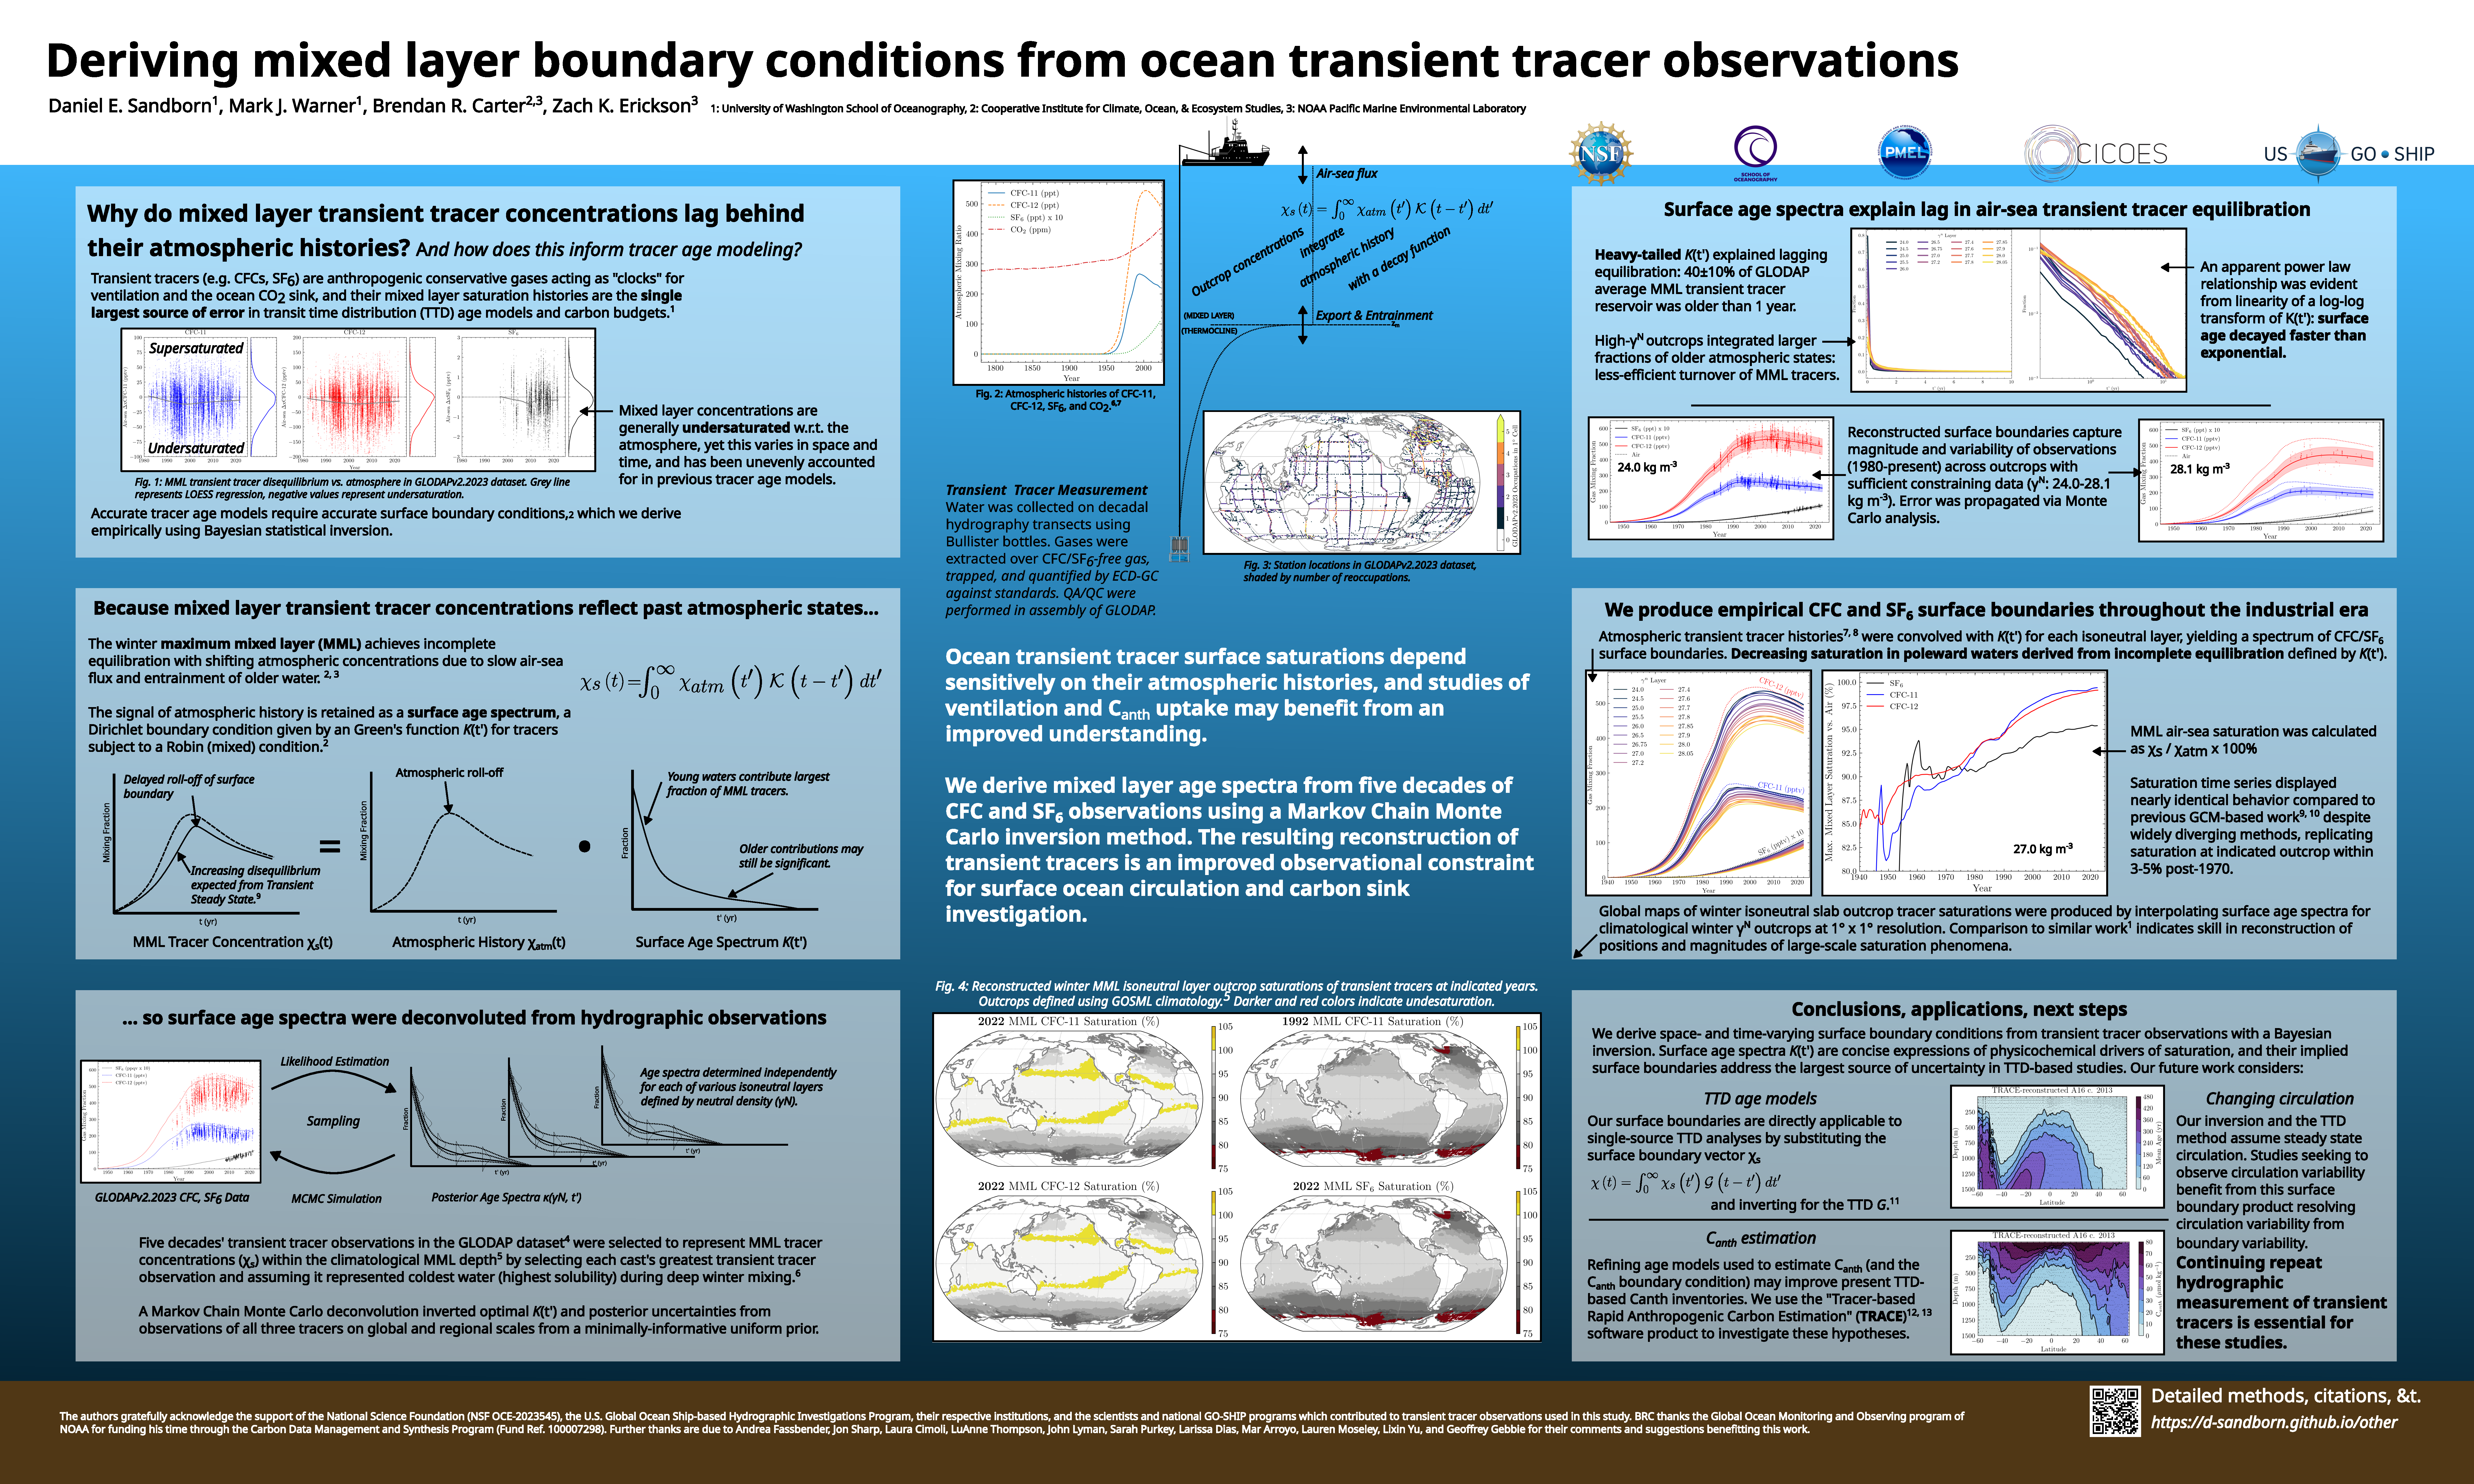
\includegraphics[width=1\linewidth,height=\textheight,keepaspectratio]{agu25_sandborn.pdf}

\subsection[Dissertations in Chemical Oceanography (DISCO XXIX)
2024]{\texorpdfstring{Dissertations in Chemical Oceanography (DISCO
XXIX)
2024\sidenote{\footnotesize \protect\pandocbounded{\includegraphics[keepaspectratio]{jgrg23094-fig-0006-m.png}}}}{Dissertations in Chemical Oceanography (DISCO XXIX) 2024}}\label{dissertations-in-chemical-oceanography-disco-xxix-20244}

\emph{Lihue, HI, USA}

``The Other CO2 problem and the Laurentian Great Lakes''

Slides available upon request. This presentation is associated with my
\href{https://hdl.handle.net/11299/270067}{doctoral dissertation} and
two of its published chapters
\href{https://doi.org/10.1029/2023JG007877}{here} and
\href{https://doi.org/10.1029/2024JG008610}{here}.

\subsection{ASLO 2024}\label{aslo-2024}

\emph{Madison, WI, USA}

``Patterns of Lake Superior AIS dispersal illustrated by particle
tracking''\sidenote{\footnotesize Associated with a manuscript:
  \endgraf
  \textbf{Sandborn, D. E.}; Austin, J. A.; Lafrancois, B. M. (2025).
  ``Developing a particle tracking model in Lake Superior'\,'. NPS
  Reports. \emph{In production.}{]}}

\subsection{OCB 2023}\label{ocb-2023}

\emph{Woods Hole, MA, USA}

``The Other CO2 Problem in the Saltless Seas: High-Resolution
Observations in Lake Superior''\sidenote{\footnotesize Associated with a publication:
  \endgraf
  \textbf{Sandborn, D. E.} \& Minor, E. C. (2024). Underway \emph{p}CO2
  surveys unravel CO2 invasion of Lake Superior from seasonal
  variability. Journal of Geophysical Research: Biogeosciences, 129,
  e2023JG007877.
  \href{https://doi.org/10.1029/2023JG007877}{doi:10.1029/2023JG007877}}

\includegraphics[width=1\linewidth,height=\textheight,keepaspectratio]{Sandborn_OCB_23.pdf}

\section{Code}\label{code}

\subsection{TRACE}\label{trace}

TRACE: Tracer-based Rapid Anthropogenic Carbon Estimation is an
algorithm for estimation of anthropogenic carbon in the ocean. It's
available for
\href{https://github.com/BRCScienceProducts/TRACEv1}{MATLAB}\sidenote{\footnotesize See
  the \href{https://doi.org/10.5194/essd-17-3073-2025}{TRACEv1 paper}.}
and \href{https://github.com/d-sandborn/pyTRACE}{Python}. For further
information on installation and use, please reference
\href{https://d-sandborn.github.io/TRACE/}{the online documentation}.

\subsection{LGLParticleTracking}\label{lglparticletracking}

\href{https://github.com/d-sandborn/LGLParticleTracking}{Demo code} for
replicating and extending our Lake Superior particle tracking study.
This work is the first to couple the updated Lake Superior Operational
Forecast System FVCOM hydrodynamic hindhast model with particle tracking
software (here, the open-source
\href{https://oceantracker.github.io/oceantracker/index.html}{OceanTracker}).
This project is described further in an NPS Report currently in
production.

\subsection{RPi-Alkalinity}\label{rpi-alkalinity}

\href{https://github.com/d-sandborn/RPi-Alkalinity}{Resources} for
open-source, low-cost alkalinity titration with a Raspberry Pi. This
project is described further in the
\href{https://aslopubs.onlinelibrary.wiley.com/doi/abs/10.1002/lom3.10549}{associated
publication}.

\section{Outreach and Teaching}\label{outreach-and-teaching}

\subsection{Day of {[}Water{]} Data 2023}\label{day-of-water-data-2023}

\href{https://d-sandborn.github.io/DayOfWaterData2023/}{A demonstration}
of data science tools applied to local water resources research.

\subsection{WikiProject Limnology and
Oceanography}\label{wikiproject-limnology-and-oceanography}

\href{https://en.wikipedia.org/wiki/Wikipedia:WikiProject_Limnology_and_Oceanography}{A
collaborative effort} to improve L\&O-related content on Wikipedia.

\bookmarksetup{startatroot}

\chapter{Contact Information}\label{contact-information}

Daniel E. Sandborn, Ph.D.\\

sandborn {[}at{]} uw.edu~

Ocean Sciences Building, 1492 NE Boat St, Seattle, WA 98105 USA\\


\backmatter
\newsavebox\mytempbib
\savebox\mytempbib{\parbox{\textwidth}{\bibliography{references.bib}}}





\end{document}
